




\documentclass[a4paper]{article}

\usepackage[english]{babel}
\usepackage[utf8]{inputenc}
\usepackage{amsthm} 
\usepackage{graphicx}
\usepackage[colorinlistoftodos]{todonotes}
\usepackage{mathtools}
\usepackage{multirow}
\usepackage{tikz}
\usepackage{qtree}
\usepackage{tikz-qtree}
\usepackage[document]{ragged2e}
\usepackage{easylist}
\usepackage{amsfonts}
\usepackage{changepage}
\usepackage{fancybox}
\title{Material dialogues for Belief Revision}
\date{}
\usepackage {mathtools}
\usepackage{lipsum}
\usepackage{easylist}
\usepackage{changepage}
\usepackage{multirow}
\usepackage{multicol}

\begin{document}
\section{Examples of Pebblings}
\subsection{}
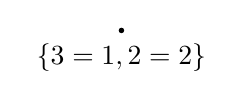
\begin{tikzpicture} 
\tikzstyle{mydot} = [circle, minimum width = 2 pt, fill, inner sep = 0 pt]  
\tikzset{every tree node/.style={mydot}, edge from parent/.append style={<-}} 
\Tree [ .\node [ mydot, label = below: {$\{3=1, 2=2\}$} ] {} ; ]
\end{tikzpicture}
\vskip 0,2 cm
\subsection{}
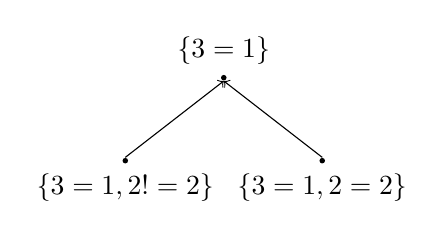
\begin{tikzpicture} 
\tikzstyle{mydot} = [circle, minimum width = 2 pt, fill, inner sep = 0 pt]  
\tikzset{every tree node/.style={mydot}, edge from parent/.append style={<-}} 
\Tree [ .\node [ mydot, label = above: {$\{3=1\}$} ] {} ;
 [.\node [ mydot, label = below: {$\{3=1, 2!=2\}$}  ] {}; ]  [.\node [ mydot, label = below: {$\{3=1, 2=2\}$}  ] {}; ] ]

\end{tikzpicture}
\subsection{}
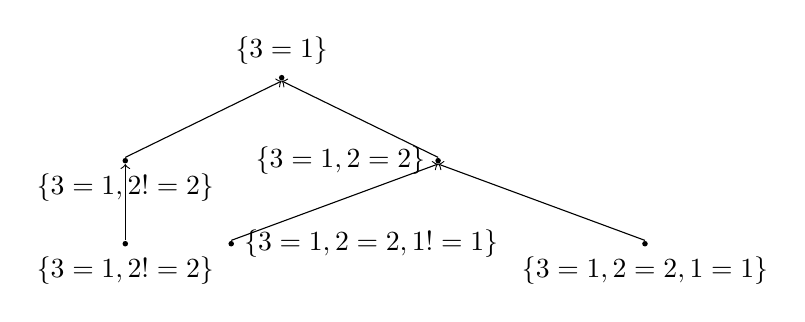
\begin{tikzpicture} 
\tikzstyle{mydot} = [circle, minimum width = 2 pt, fill, inner sep = 0 pt]  
\tikzset{every tree node/.style={mydot}, edge from parent/.append style={<-}} 
\Tree [ .\node [ mydot, label = above: {$\{3=1\}$} ] {} ;
 [.\node [ mydot, label = below: {$\{3=1, 2!=2\}$}  ] {};  [ .\node [ mydot, label = below: {$\{3=1, 2!=2\}$}  ] {};  ] ]  [.\node [ mydot, label = left: {$\{3=1, 2=2\}$}  ] {}; [ .\node [ mydot, label = right: {$\{3=1, 2=2, 1!=1 \}$}  ] {}; ] [ .\node [ mydot, label = below: {$\{3=1, 2=2, 1=1 \}$}  ] {}; ]  ] ]
 
\end{tikzpicture}

\end{document}



